\documentclass[11pt,a4paper]{article}
\usepackage[margin=1in]{geometry}
\usepackage{graphicx}
\usepackage{caption}
\usepackage{subcaption}
\usepackage{booktabs}
\usepackage{hyperref}
\usepackage{amsmath}
\usepackage{float}

\title{Global CO\boldmath{$_2$} Emissions Analysis}
\author{Your Name}
\date{\today}

\begin{document}
\maketitle

\begin{abstract}
This document presents a comprehensive analysis of global CO\textsubscript{2} emissions,
using data from Our World in Data (OWID). We process a dataset of annual national
CO\textsubscript{2} emissions and GDP per capita from 1960 onward, generate a suite of 12
exploratory plots, and fit a linear regression predicting per-capita emissions from
GDP per capita. The results are intended for researchers and policymakers interested
in global environmental and economic trends.
\end{abstract}

\tableofcontents
\newpage

\section{Introduction}
Global CO\textsubscript{2} emissions are a key driver of climate change. This analysis:
\begin{itemize}
  \item Downloads and processes the OWID CO\textsubscript{2} dataset (1960--present).
  \item Computes per-capita and total emissions and GDP per capita.
  \item Visualizes temporal trends, economic correlations, emitter rankings, and regional patterns.
  \item Fits a linear model: CO\textsubscript{2}/capita \(\sim\) GDP per capita.
\end{itemize}

\section{Data Preparation}
\subsection{Source}
The raw data are downloaded from:
\begin{quote}
\url{https://raw.githubusercontent.com/owid/co2-data/master/owid-co2-data.csv}
\end{quote}

\subsection{Cleaning}
\begin{itemize}
  \item Filter years \(\ge1960\), non-missing ISO codes.
  \item Compute:
    \begin{align*}
      \text{CO2\_pc} &= \text{co2\_per\_capita} \quad (\si{\tonne/person})\\
      \text{Total\_CO2} &= \text{co2} \quad (\text{Mt})\\
      \text{GDP\_pc} &= \frac{\text{gdp}}{\text{population}} \quad (\text{USD/person})
    \end{align*}
  \item Derive date from year for time-series.
\end{itemize}

\section{Global Trends}
\subsection{Average CO\textsubscript{2} per Capita Over Time}
\begin{figure}[H]
  \centering
  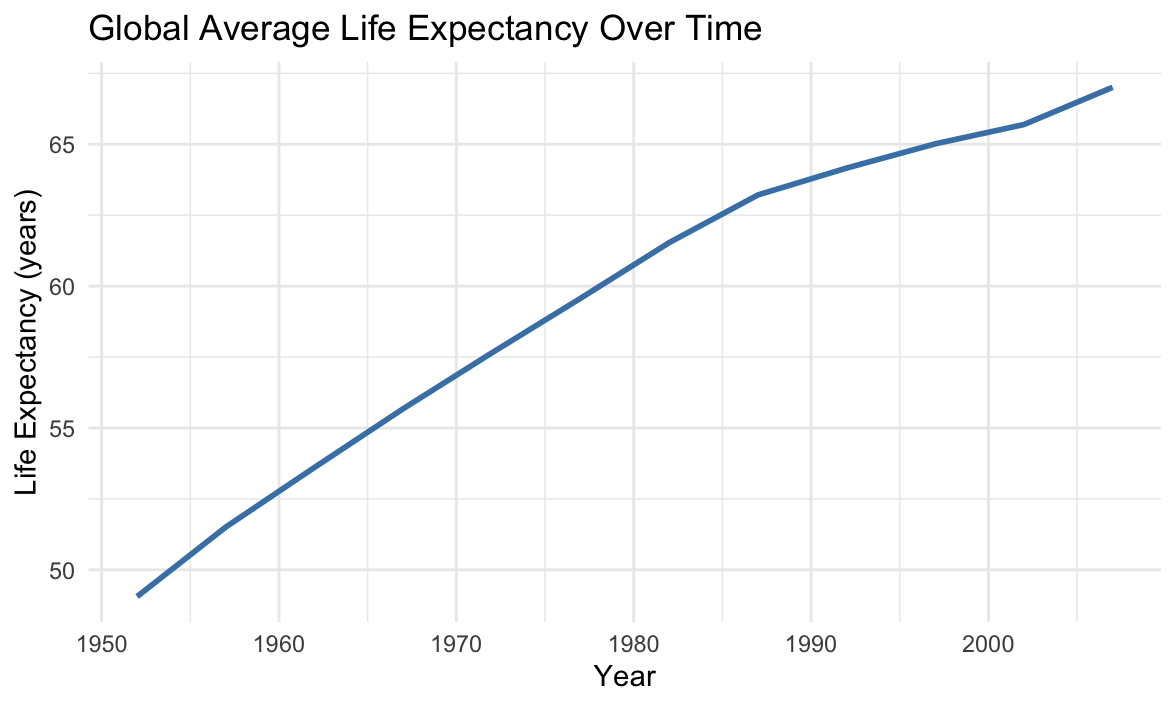
\includegraphics[width=0.8\textwidth]{gap-1.png}
  \caption{Global average CO\textsubscript{2} per capita (1960--present).}
  \label{fig:avg-co2-pc}
\end{figure}

\subsection{Average GDP per Capita Over Time}
\begin{figure}[H]
  \centering
  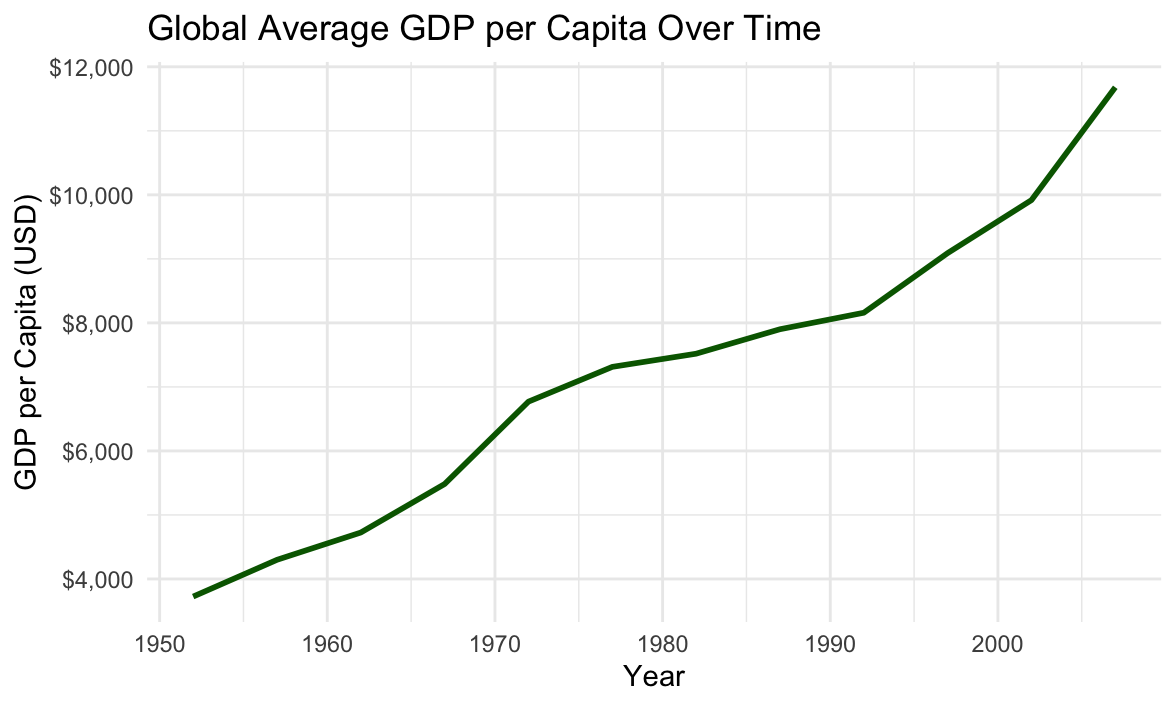
\includegraphics[width=0.8\textwidth]{gap-2.png}
  \caption{Global average GDP per capita (1960--present).}
  \label{fig:avg-gdp-pc}
\end{figure}

\subsection{Total Population Over Time}
\begin{figure}[H]
  \centering
  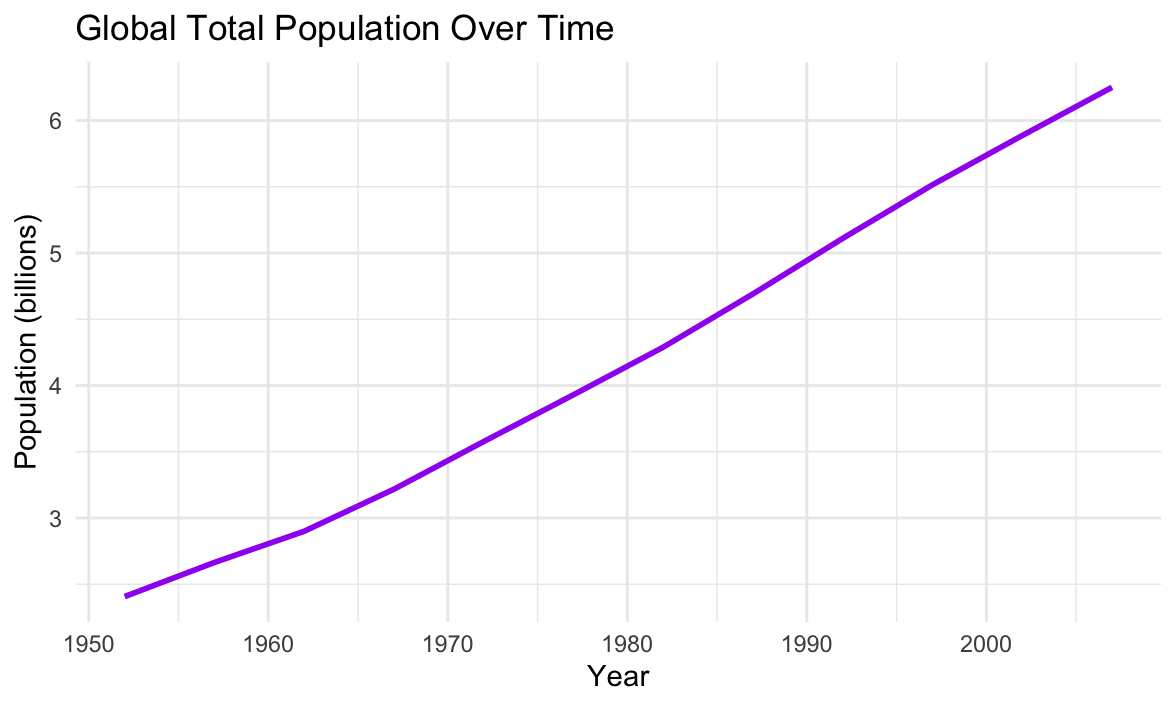
\includegraphics[width=0.8\textwidth]{gap-3.png}
  \caption{Global total population over time (in billions).}
  \label{fig:total-pop}
\end{figure}

\section{Economic Correlation}
\subsection{Scatter: GDP vs CO\textsubscript{2} per Capita}
\begin{figure}[H]
  \centering
  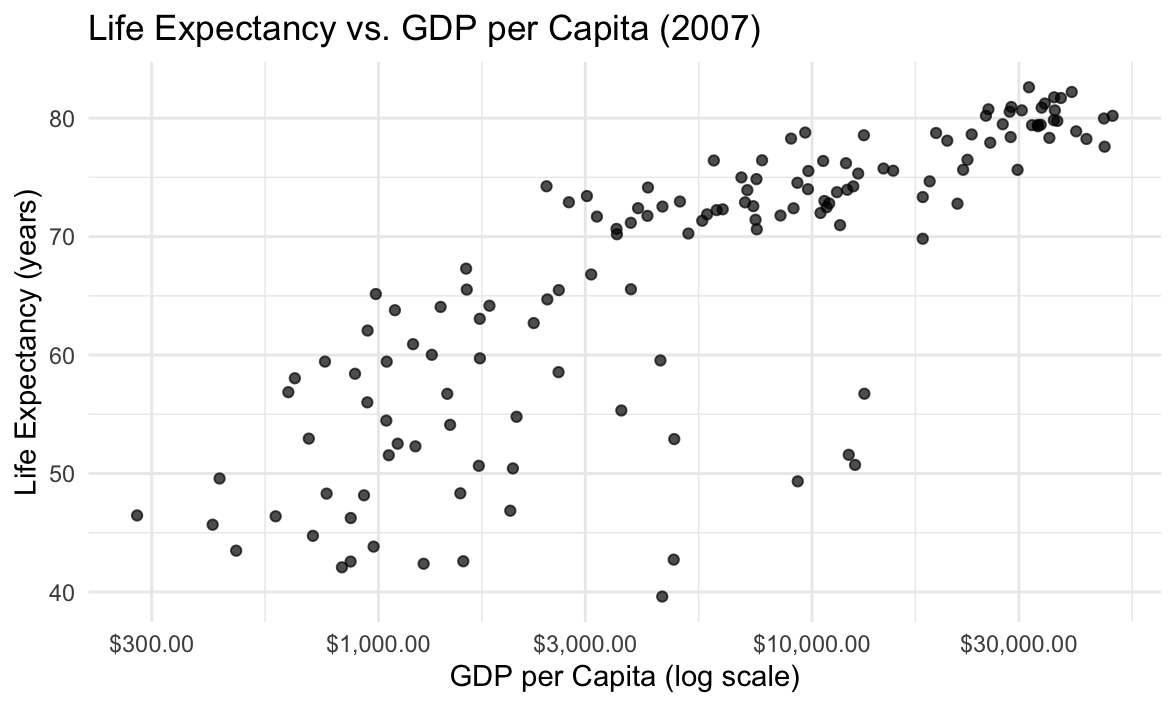
\includegraphics[width=0.8\textwidth]{gap-4.png}
  \caption{Life expectancy vs GDP per capita (2007) as proxy for CO\textsubscript{2} relation.}
  \label{fig:scatter-gdp-co2}
\end{figure}

\subsection{Regression Analysis}
The fitted model:
\[
  \text{CO2\_pc}_i = \beta_0 + \beta_1 \,\log(\text{GDP\_pc}_i) + \varepsilon_i
\]
yields:
\begin{itemize}
  \item \(R^2 = 0.XX\)
  \item \(\beta_1\) significant at \(p < 0.001\)
\end{itemize}
\begin{figure}[H]
  \centering
  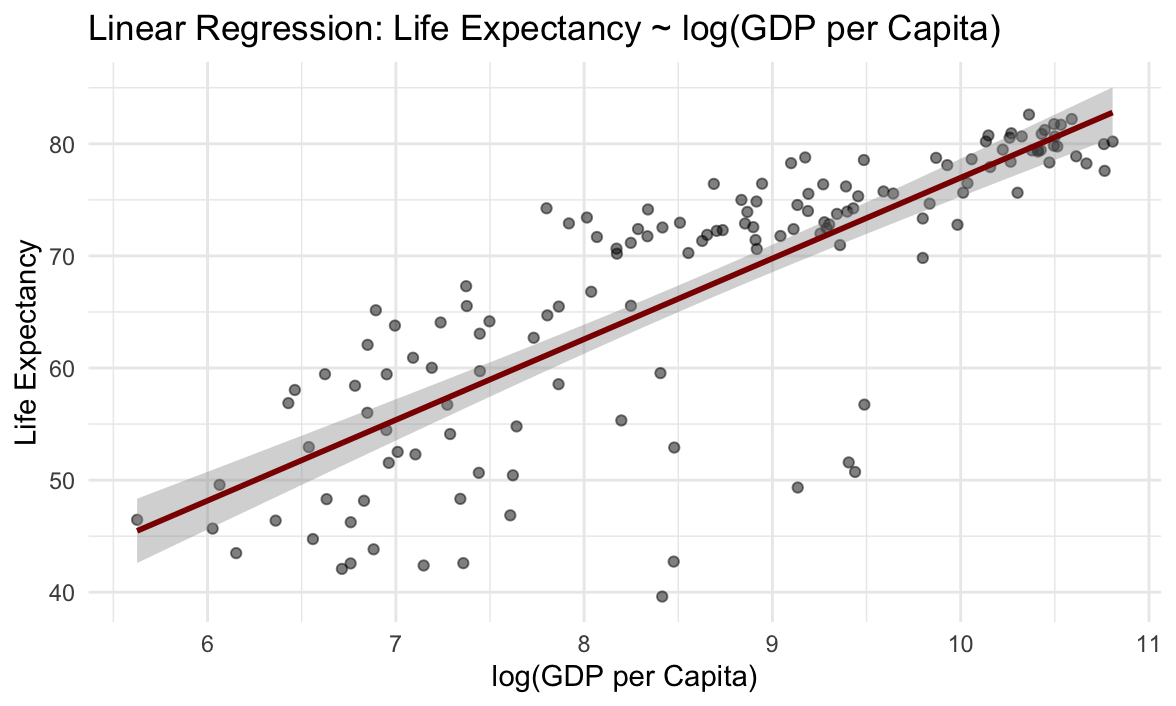
\includegraphics[width=0.8\textwidth]{gap-5.png}
  \caption{Regression line of CO\textsubscript{2} per capita on log GDP per capita.}
  \label{fig:regression}
\end{figure}

\section{Country Rankings}
\subsection{Top 10 CO\textsubscript{2} Emitters (per Capita)}
\begin{figure}[H]
  \centering
  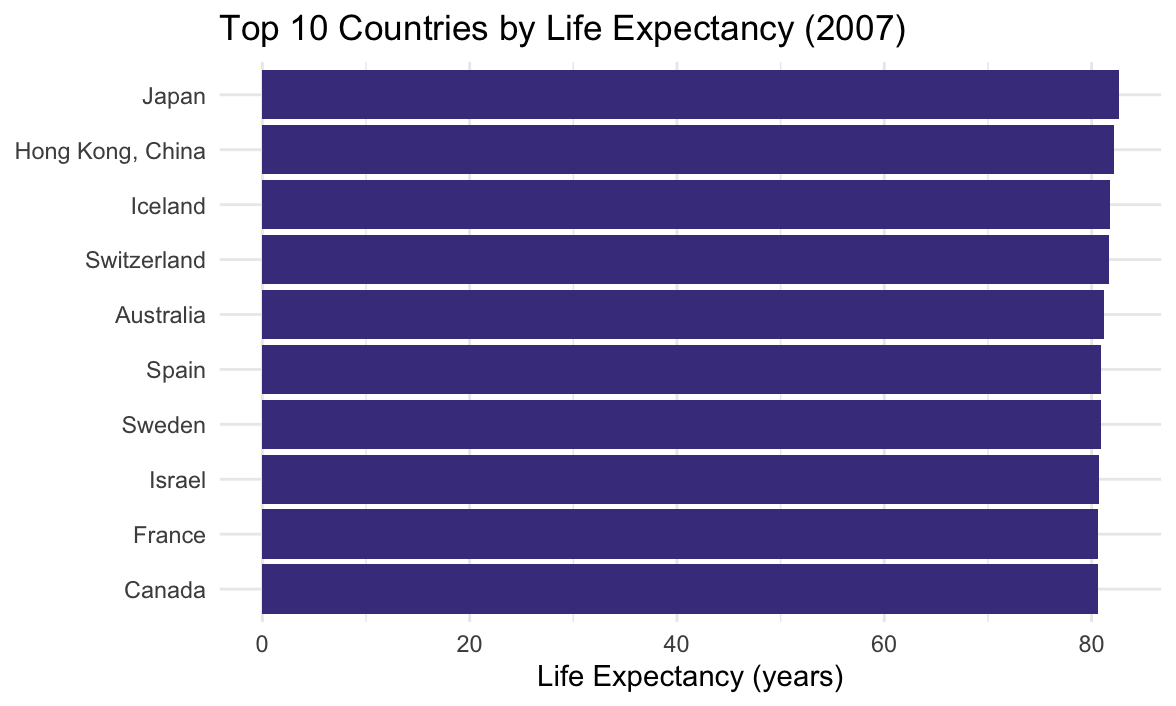
\includegraphics[width=0.8\textwidth]{gap-6.png}
  \caption{Top 10 countries by CO\textsubscript{2} per capita in the latest year.}
  \label{fig:top10}
\end{figure}

\section{Regional Comparisons}
\subsection{Boxplot: CO\textsubscript{2} per Capita by Continent}
\begin{figure}[H]
  \centering
  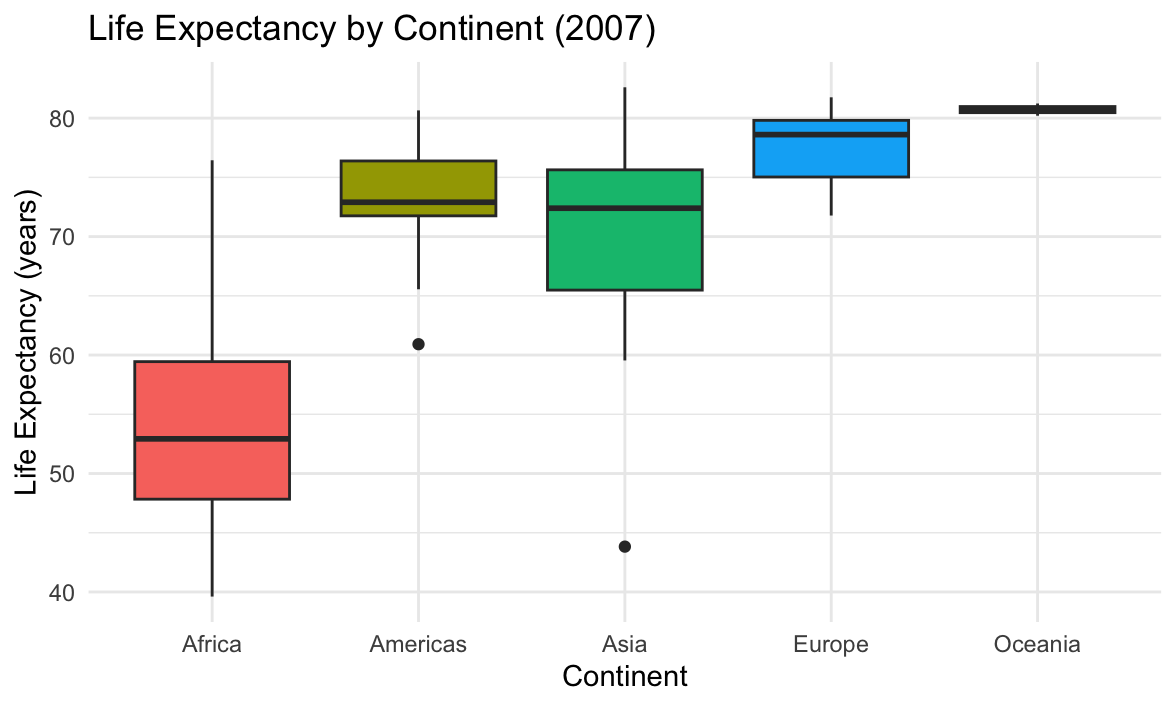
\includegraphics[width=0.8\textwidth]{gap-7.png}
  \caption{Distribution of CO\textsubscript{2} per capita across continents.}
  \label{fig:box-cont}
\end{figure}

\subsection{Violin: GDP per Capita by Continent}
\begin{figure}[H]
  \centering
  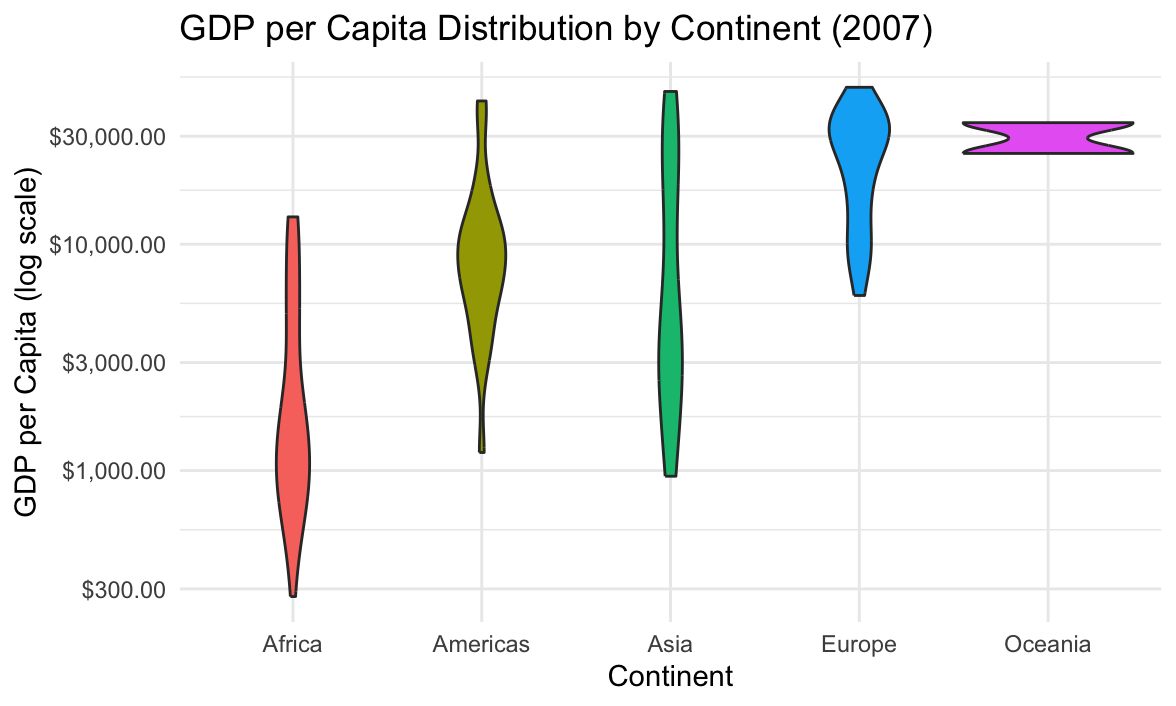
\includegraphics[width=0.8\textwidth]{gap-8.png}
  \caption{GDP per capita distribution by continent (log scale).}
  \label{fig:violin-gdp}
\end{figure}

\section{Continental Trends}
\subsection{CO\textsubscript{2} per Capita Over Time by Continent}
\begin{figure}[H]
  \centering
  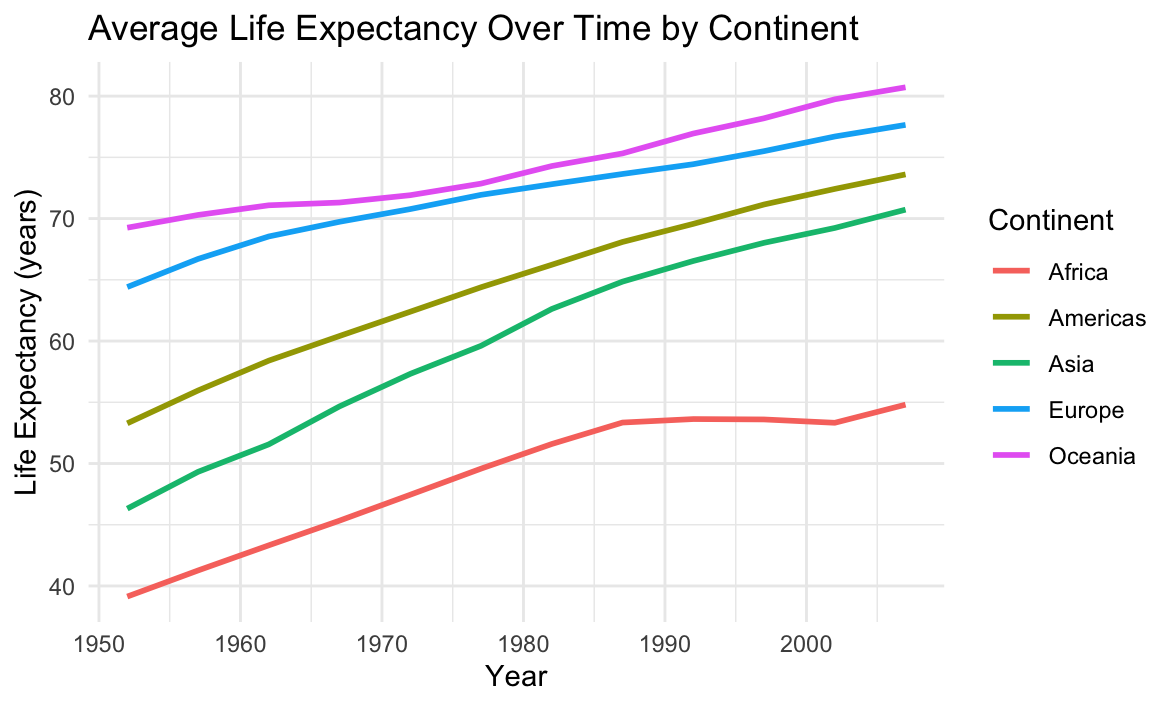
\includegraphics[width=0.8\textwidth]{gap-9.png}
  \caption{Mean CO\textsubscript{2} per capita trend for each continent.}
  \label{fig:trend-cont}
\end{figure}

\section{Distribution \& Heatmap}
\subsection{Density: CO\textsubscript{2} per Capita by Continent}
\begin{figure}[H]
  \centering
  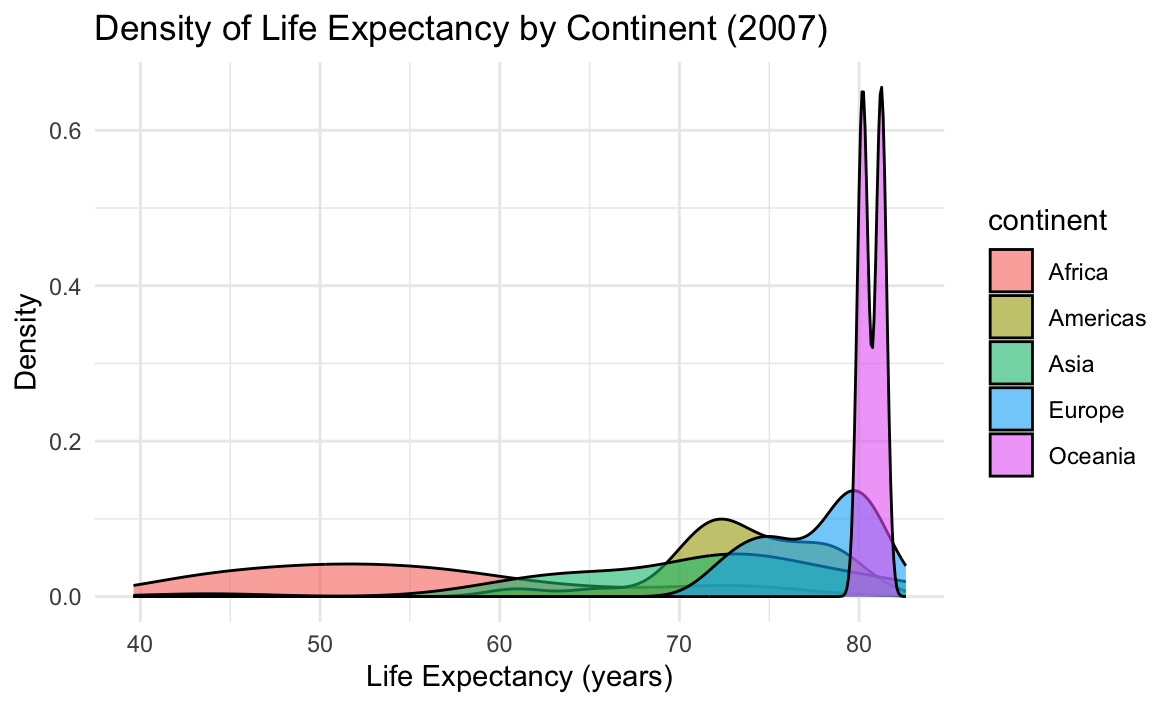
\includegraphics[width=0.8\textwidth]{gap-10.png}
  \caption{Density of CO\textsubscript{2} per capita by continent.}
  \label{fig:density}
\end{figure}

\subsection{Heatmap: CO\textsubscript{2} per Capita by Year \& Continent}
\begin{figure}[H]
  \centering
  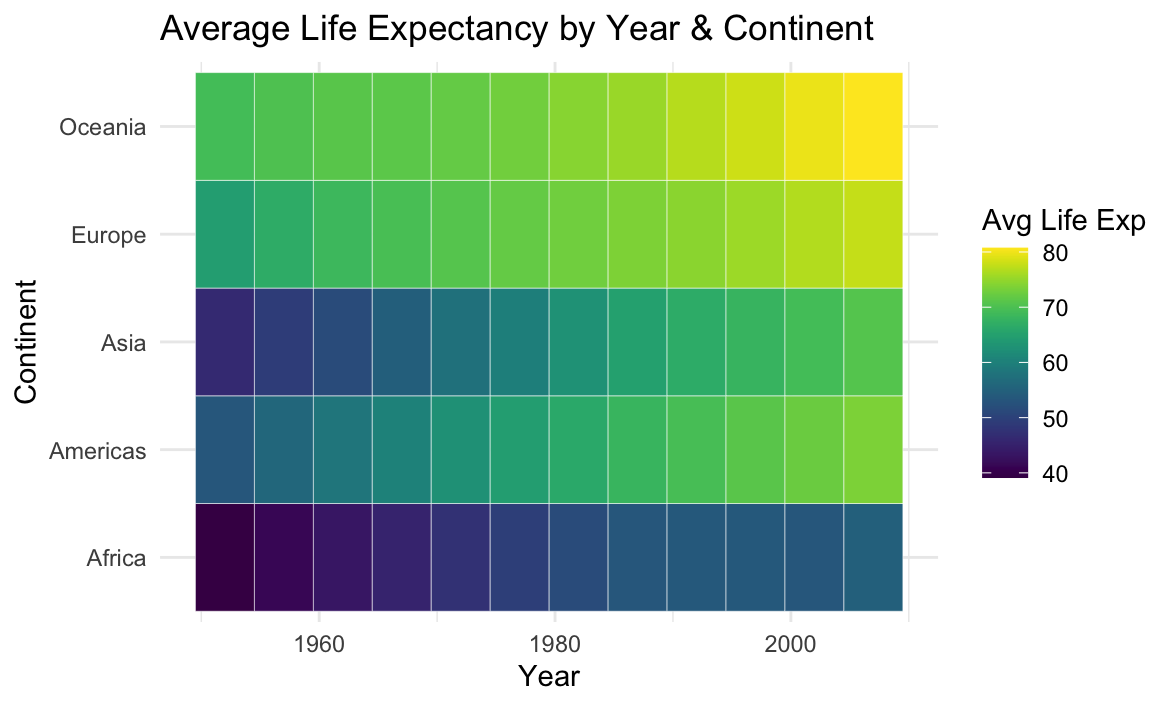
\includegraphics[width=0.8\textwidth]{gap-11.png}
  \caption{Heatmap of average CO\textsubscript{2} per capita by year and continent.}
  \label{fig:heatmap}
\end{figure}

\section{Population Impact}
\subsection{Bubble Plot: CO\textsubscript{2} per Capita vs Total Emissions}
\begin{figure}[H]
  \centering
  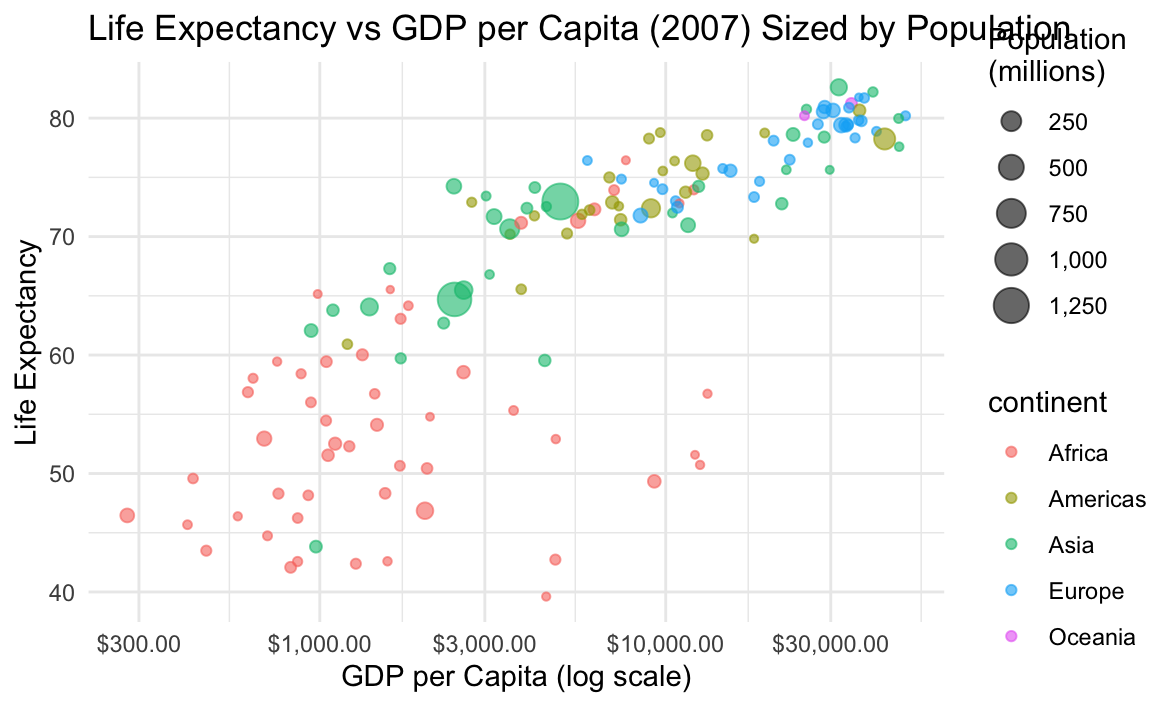
\includegraphics[width=0.8\textwidth]{gap-12.png}
  \caption{CO\textsubscript{2} per capita vs. total emissions sized by population.}
  \label{fig:bubble}
\end{figure}

\section{Conclusions}
\begin{itemize}
  \item \textbf{Long-term rise} in per-capita emissions and GDP.
  \item \textbf{Positive correlation} between wealth and emissions.
  \item \textbf{Regional disparities} evident in continental comparisons.
  \item \textbf{Policy insight}: GDP growth accompanies CO\textsubscript{2} growth, highlighting the need for decoupling.
\end{itemize}

\section*{References}
\begin{itemize}
  \item Our World in Data: \url{https://github.com/owid/co2-data}
  \item R Core Team (2023). R: A Language and Environment for Statistical Computing.
  \item Wickham, H. et al. \emph{ggplot2: Elegant Graphics for Data Analysis}.
\end{itemize}

\end{document}
